% Machine Learning (notes), in unconventional ``grande'' format; fitting a widescreen format
% 
% github        : ernestyalumni
% gmail         : ernestyalumni 
% linkedin      : ernestyalumni 
% wordpress.com : ernestyalumni
%
% This code is open-source, governed by the Creative Common license.  Use of this code is governed by the Caltech Honor Code: ``No member of the Caltech community shall take unfair advantage of any other member of the Caltech community.'' 

\documentclass[10pt]{amsart}
\pdfoutput=1
%\usepackage{mathtools,amssymb,lipsum,caption}
\usepackage{mathtools,amssymb,caption}


\usepackage{graphicx}
\usepackage{hyperref}
\usepackage[utf8]{inputenc}
\usepackage{listings}
\usepackage[table]{xcolor}
\usepackage{pdfpages}
\usepackage{tikz}
\usetikzlibrary{matrix,arrows,backgrounds}

\usepackage{multicol}

\hypersetup{colorlinks=true,citecolor=[rgb]{0,0.4,0}}

\oddsidemargin=15pt
\evensidemargin=5pt
\hoffset-45pt
\voffset-55pt
\topmargin=-4pt
\headsep=5pt
\textwidth=1120pt
\textheight=595pt
\paperwidth=1200pt
\paperheight=700pt
\footskip=40pt

\newtheorem{theorem}{Theorem}
\newtheorem{corollary}{Corollary}
%\newtheorem*{main}{Main Theorem}
\newtheorem{lemma}{Lemma}
\newtheorem{proposition}{Proposition}

\newtheorem{definition}{Definition}
\newtheorem{remark}{Remark}

\newenvironment{claim}[1]{\par\noindent\underline{Claim:}\space#1}{}
\newenvironment{claimproof}[1]{\par\noindent\underline{Proof:}\space#1}{\hfill $\blacksquare$}

%This defines a new command \questionhead which takes one argument and
%prints out Question #. with some space.
\newcommand{\questionhead}[1]
  {\bigskip\bigskip
   \noindent{\small\bf Question #1.}
   \bigskip}

\newcommand{\problemhead}[1]
  {
   \noindent{\small\bf Problem #1.}
   }

\newcommand{\exercisehead}[1]
  { \smallskip
   \noindent{\small\bf Exercise #1.}
  }

\newcommand{\solutionhead}[1]
  {
   \noindent{\small\bf Solution #1.}
   }

\title{Deep Learning}
\author{Ernest Yeung \href{mailto:ernestyalumni@gmail.com}{ernestyalumni@gmail.com}}
\date{22 November 2023}
\keywords{Machine Learning, statistical inference, statistical inference learning, deep learning}
\begin{document}

\definecolor{darkgreen}{rgb}{0,0.4,0}
\lstset{language=C++,
  keywordstyle=\color{blue},
  stringstyle=\color{red},
 commentstyle=\color{darkgreen}
 }
%\lstlistoflistings

\maketitle


From the beginning of 2016, I decided to cease all explicit crowdfunding for any of my materials on physics, math.  I failed to raise \emph{any} funds from previous crowdfunding efforts.  I decided that if I was going to live in \emph{abundance}, I must lose a scarcity attitude.  I am committed to keeping all of my material \textbf{open-sourced}.  I give all my stuff \emph{for free}.   

In the beginning of 2017, I received a very generous donation from a reader from Norway who found these notes useful, through \emph{PayPal}.  If you find these notes useful, feel free to donate directly and easily through \href{https://www.paypal.com/cgi-bin/webscr?cmd=_donations&business=ernestsaveschristmas%2bpaypal%40gmail%2ecom&lc=US&item_name=ernestyalumni&currency_code=USD&bn=PP%2dDonationsBF%3abtn_donateCC_LG%2egif%3aNonHosted}{PayPal}, which won't go through a 3rd. party such as indiegogo, kickstarter, patreon.  Also, you can donate to me on \href{https://venmo.com/ernestyalumni}{Venmo}, Otherwise, under the \emph{open-source MIT license}, feel free to copy, edit, paste, make your own versions, share, use as you wish.    

\noindent gmail        : ernestyalumni \\
linkedin     : ernestyalumni \\
tumblr       : ernestyalumni \\
twitter      : ernestyalumni \\
youtube      : ernestyalumni \\

\tableofcontents

\begin{multicols*}{2}

\begin{abstract}
Everything about Machine Learning, Deep Learning.  
\end{abstract}

\part{Neural Networks}

\section{Loss functions}

\subsection{L1}

From Pytorch Docs, torch.nn,
\href{https://pytorch.org/docs/stable/generated/torch.nn.L1Loss.html#torch.nn.L1Loss}{L1Loss Pytorch}

\[
\begin{gathered}
	\ell(x, y) = L = \{l_1,\dots,l_N\}^\top, \quad
	l_n = \left| x_n - y_n \right|
\end{gathered}
\]
	
	where \( N \) is the batch size. If `reduction` is not `'none'`
	(default `'mean'`), then:

\[
\begin{gathered}	
	\ell(x, y) =
	\begin{cases}
		\operatorname{mean}(L), & \text{if reduction} = \text{`mean';}\\
		\operatorname{sum}(L),  & \text{if reduction} = \text{`sum'.}
	\end{cases}
\end{gathered}
\]

Instead, consider the following: let $\mathbf{x}, \mathbf{y} \in \mathbf{R}^N$ where $\mathbf{R}$ is some ring (integers and floating point types in computer sciecne are at least rings).

Let $\mathbf{x}$ be the predicted values and $\mathbf{y}$ be the true values.

If 
\[
l(x,y) = L = \lbrace l_1, \dots l_N \rbrace^T, \, l_n = |x_n - y_n|
\]
then
\[
\frac{\partial }{ \partial x^i} L = \frac{\partial}{\partial x^i} \begin{cases} x_j - y_j & \text{ if } x_j \geq y_j \\ y_j -x_j & \text{ if } x_j < y_j \end{cases} = \begin{cases} 1 & \text{ if } x_j \geq y_j \\ -1 & \text{ if } x_j < y_j \end{cases}
\]

If 
\[
l(x,y) = L = \frac{1}{N} \sum_{j=1}^N l_j 
\]
Then
\[
\frac{\partial }{ \partial x_i} L = \frac{1}{N} \begin{cases} 1 & \text{ if } x_j \geq y_j \\
	-1 & \text{ if } x_j < y_j \end{cases}
\]

If 
\[
l(x,y) = L =  \sum_{j=1}^N l_j 
\]
Then
\[
\frac{\partial }{ \partial x_i} L =  \begin{cases} 1 & \text{ if } x_j \geq y_j \\
	-1 & \text{ if } x_j < y_j \end{cases}
\]

\part{CUDA}

Keep in mind that CUDA won't be the end-all, be-all for optimized deep learning. Consider Open XLA and consider LLVM.

\section{Threads, Blocks, Grids}

cf. Chapter 5 Thread Cooperation, Section 5.2. Splitting Parallel Blocks of Sanders and Kandrot (2010) \cite{SK2010}.

Consider first a 1-dimensional block.

\begin{itemize}
	\item \verb|threadIdx.x| $\Longleftarrow$ $M_x \equiv $ number of threads per block in $x$-direction.  Let $j_x = 0 \dots M_x-1$ be the index for the thread.  Note that $1 \leq M_x \leq M_x^{\text{max}}$, where $M_x^{\text{max}} = 1024$ is the maximum number of threads per block that can be allocated, which is a hard hardware limit (I presume). 
	\item \verb|blockIdx.x| $\Longleftarrow$ $N_x \equiv $ number of blocks in $x$-direction.  Let $i_x = 0\dots N_x-1$
	\item \verb|blockDim| stores number of threads along each dimension of the block $M_x$.  
\end{itemize}

Then if we were to ``linearize'' or ``flatten'' in this $x$-direction,
\begin{equation}\label{Eq:GlobalIndexCUDA1Dim}
k = j_x + i_x M_x
\end{equation}
where $k$ is the $k$th thread.  $k=0\dots N_xM_x -1$.

Take a look at \href{https://github.com/ernestyalumni/CompPhys/blob/master/CUDA-By-Example/heattexture1.cu}{heattexture1.cu} which uses the GPU texture memory.  Look at how \verb|threadIdx|/\verb|blockIdx| is mapped to pixel position.

As an exercise, let's again rewrite the code in mathematical notation:
\begin{itemize}\label{List:threadblockdict}
	\item \verb|threadIdx.x| $\Longleftarrow j_x$, $0\leq j_x \leq M_x -1$ 
	\item \verb|blockIdx.x| $\Longleftarrow i_x$, $0\leq i_x \leq N_x -1$
	\item \verb|blockDim.x| $\Longleftarrow M_x$, number of threads along each dimension (here dimension $x$) of a block, $1 \leq M_x \leq M_x^{\text{max}} = 1024$
	\item \verb|gridDim.x| $\Longleftarrow N_x$, $1\leq N_x$
\end{itemize}
resulting in
\begin{itemize}
	\item $k_x = j_x +i_x M_x$ $\Longrightarrow$
	\begin{lstlisting}
		int x =  threadIdx.x + blockIdx.x * blockDim.x ;
	\end{lstlisting}
	\item $k_y = j_y +i_y M_y$ $\Longrightarrow$
	\begin{lstlisting}
		int y =  threadIdx.y + blockIdx.y * blockDim.y ;
	\end{lstlisting}
\end{itemize}
and so for a ``flattened'' thread index $J \in \mathbb{N}$,
\[
J = k_x + N_x\cdot M_x \cdot k_y
\]
$\Longrightarrow $
\begin{lstlisting}
	offset = x + y * blockDim.x * gridDim.x ;
\end{lstlisting}

Suppose vector is of length $N$.  So we \emph{need} $N$ parallel threads to launch, in total. \\
e.g. if $M_x = 128$ threads per block, $N/128 = N/M_x$ blocks to get our total of $N$ threads running.

Wrinkle: integer division!  e.g. if $N=127 $, $\frac{N}{128} = 0$.

Solution: consider $\frac{N+127}{128}$ blocks.  If $N = l\cdot 128 + r$, $l\in \mathbb{N}$, $r = 0 \dots 127$.
\[
\begin{gathered}
	\frac{N+127}{128} = \frac{ l \cdot 128 + r + 127 }{128} = \frac{ (l+1)128 + r- 1}{128} = \\
	= l+1 + \frac{r-1}{128} = \begin{cases}
		l & \text{ if } r= 0 \\
		l+1 & \text{ if } r = 1 \dots 127
	\end{cases}
\end{gathered}
\]
\[
\begin{gathered}
	\frac{ N + (M_x - 1) }{M_x} = \frac{ l\cdot M_x + r+ M_x - 1}{M_x} = \frac{ (l+1)M_x + r-1 }{M_x} = \\
	= l+1 + \frac{r-1}{M_x} = \begin{cases}
		l & \text{ if } r = 0 \\
		l +1 & \text{ if } r = 1 \dots M_x -1 
	\end{cases}
\end{gathered}
\]

So $\frac{N+(M_x-1)}{M_x}$ is the smallest multiple of $M_x$ greater than or equal to $N$, so $\frac{N + (M_x- 1)}{M_x}$ \textbf{blocks are needed or more than needed to run a total of $N$ threads.}


Problem: Max. grid dim. in 1-direction is 65535, $\equiv N_i^{\text{max}}$.

So $\frac{ N+ (M_x-1)}{M_x} = N_i^{\text{max}} \Longrightarrow N = N_i^{\text{max}} M_x - (M_x-1) \leq N_i^{\text{max}} M_x$.  i.e. number of threads $N$ is limited by $N_i^{\text{max}} M_x$.

Solution.

\begin{itemize}
	\item number of threads per block in $x$-direction $\equiv M_x \Longrightarrow $ \verb|blockDim.x| \\
	\item number of blocks in grid $\equiv N_x \Longrightarrow $ \verb|gridDim.x| 
	\item $N_x M_x$ total number of threads in $x$-direction.  Increment by $N_xM_x$.  So next scheduled execution by GPU at the $k= N_xM_x$ thread.  
\end{itemize}

Sanders and Kandrot (2010) \cite{SK2010} made an important note, on pp. 176-177 Ch. 9 Atomics of Section 9.4 Computing Histograms, an important \emph{rule of thumb} on the number of blocks.

First, consider $N^{\text{threads}}$ total threads.  The extremes are either $N^{\text{threads}}$ threads on a single block, or $N^{\text{threads}}$ blocks, each with a single thread.

Sanders and Kandrot gave this tip:  \\

number of blocks, i.e. \verb|gridDim.x| $\Longleftarrow N_x$ $\sim 2 \times $ number of GPU multiprocessors, i.e. twice the number of GPU multiprocessors.  In the case of my GeForce GTX 980 Ti, it has 22 Multiprocessors.  

\subsection{global thread Indexing: 1-dim., 2-dim., 3-dim.}

Consider the problem of \emph{global thread indexing.}  This was asked on the NVIDIA Developer's board (cf. \href{https://devtalk.nvidia.com/default/topic/498642/calculate-global-thread-id/?offset=2}{Calculate GLOBAL thread Id}).  Also, there exists a ``cheatsheet'' (cf. \href{https://cs.calvin.edu/courses/cs/374/CUDA/CUDA-Thread-Indexing-Cheatsheet.pdf}{CUDA Thread Indexing Cheatsheet}).  Let's consider a (mathematical) generalization.

Consider again (cf. \ref{List:threadblockdict}) the following notation: 
\begin{itemize}
	\item \verb|threadIdx.x| $\Longleftarrow i_x$, $0\leq i_x \leq M_x -1$, \qquad \, $i_x \in \lbrace 0 \dots M_x - 1\rbrace \equiv I_x$, of ``cardinal length/size'' of $|I_x| = M_x$
	\item \verb|blockIdx.x| $\Longleftarrow j_x$, $0\leq j_x \leq N_x -1$, \qquad \, $j_x \in \lbrace 0 \dots N_x - 1\rbrace \equiv J_x$, of ``cardinal length/size'' of $|J_x| = N_x$
	\item \verb|blockDim.x| $\Longleftarrow M_x$
	\item \verb|gridDim.x| $\Longleftarrow N_x$
\end{itemize}

Now consider formulating the various cases, of a grid of dimensions from 1 to 3, and blocks of dimensions from 1 to 3 (for a total of 9 different cases) mathematically, as the \href{https://cs.calvin.edu/courses/cs/374/CUDA/CUDA-Thread-Indexing-Cheatsheet.pdf}{CUDA Thread Indexing Cheatsheet} did, similarly:

\begin{itemize}
	\item \emph{1-dim. grid} of \emph{1-dim. blocks}.   Consider $J_x\times I_x$.  For $j_x \in J_x$, $i_x \in I_x$, then $k_x = j_x M_x + i_x$, $k_x \in \lbrace 0 \dots N_xM_x-1\rbrace \equiv K_x$.
	
	The condition that $k_x$ be a valid global thread index is that $K_x$ has equal cardinality or size as $J_x\times I_x$, i.e.
	\[
	|J_x \times I_x| = |K_x|
	\]
	(this must be true).  This can be checked by checking the most extreme, maximal, case of $j_x = N_x-1$, $i_x = M_x-1$:
	\[
	k_x = j_xM_x + i_x = (N_x-1)M_x + M_x-1 = N_xM_x -1
	\]
	and so $k_x$ ranges from $0$ to $N_xM_x-1$, and so $|K_x|=N_xM_x$.
	
	Summarizing all of this in the following manner:
	\[
	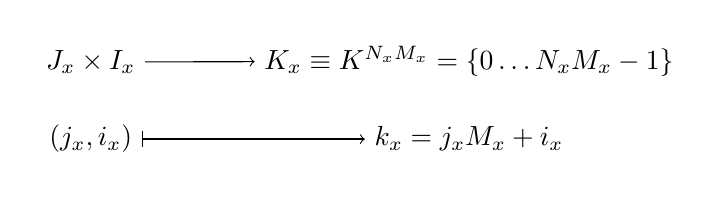
\begin{tikzpicture}
		\matrix (m) [matrix of math nodes, row sep=1.1em, column sep=4em, minimum width=1em]
		{
			J_x \times I_x &  K_x \equiv K^{N_xM_x}= \lbrace 0 \dots N_xM_x -1\rbrace \\ 
			(j_x,i_x) & k_x = j_xM_x +i_x \\ 
		};
		\path[->]
		(m-1-1) edge node [auto] {$$} (m-1-2)
		;  
		\path[|->]
		(m-2-1) edge node [auto] {$$} (m-2-2)
		;
	\end{tikzpicture} 
	\]
	
	For the other cases, this generalization we've just done is implied.  
	\item \emph{1-dim. grid} of \emph{2-dim. blocks}
	\[
	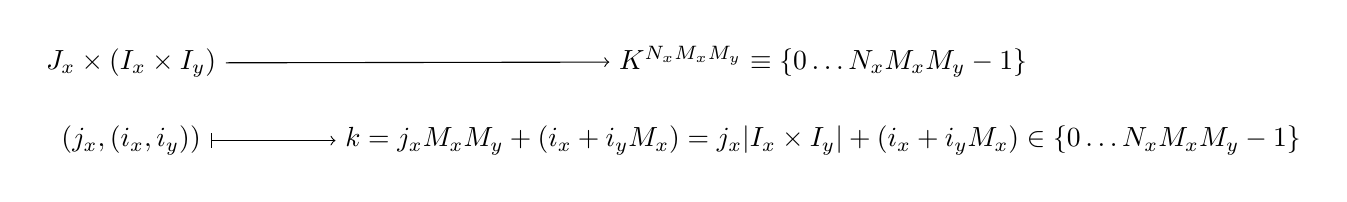
\begin{tikzpicture}
		\matrix (m) [matrix of math nodes, row sep=1.1em, column sep=4em, minimum width=1em]
		{
			J_x \times (I_x\times I_y) &  K^{N_xM_xM_y} \equiv \lbrace 0 \dots N_xM_xM_y -1\rbrace \\ 
			(j_x,(i_x,i_y)) & k = j_xM_xM_y +(i_x+i_yM_x) = j_x |I_x\times I_y| + (i_x + i_yM_x) \in \lbrace 0 \dots N_xM_xM_y -1 \rbrace \\ 
		};
		\path[->]
		(m-1-1) edge node [auto] {$$} (m-1-2)
		;  
		\path[|->]
		(m-2-1) edge node [auto] {$$} (m-2-2)
		;
	\end{tikzpicture} 
	\]
	%\[
	%\begin{gathered}
	%  (j_x,i_x)\mapsto k_x = j_xM_x + i_x
	%\end{gathered}
	%\]
	The ``most extreme, maximal'' case that can be checked to check that the ``cardinal size'' of $K^{N_xM_xM_y}$ is equal to $J_x\times (I_x\times I_y)$ is the following, and for the other cases, will be implied (unless explicitly written or checked out):
	\[
	k = j_x M_xM_y + (i_x + i_y M_x) = (N_x-1)M_xM_y + ((M_x-1) + (M_y-1)M_x) = (N_xM_xM_y-1) 
	\]
	The thing to notice is this emerging, general pattern, what could be called a ``global view'' of understanding the threads and blocks model of the GPU (cf. \href{https://devtalk.nvidia.com/default/topic/498642/calculate-global-thread-id/?offset=2}{njuffa's answer}:
	\[
	\text{ total number of threads } = \text{ block index (Id) }\cdot \text{ total number of threads per blcok } + \text{ thread index on the block }
	\]
	But as we'll see, that's not the only way of ``flattening'' the index, or transforming into a 1-dimensional index.  
	
	\item \emph{1-dim. grid} of \emph{3-dim. blocks}
	\[
	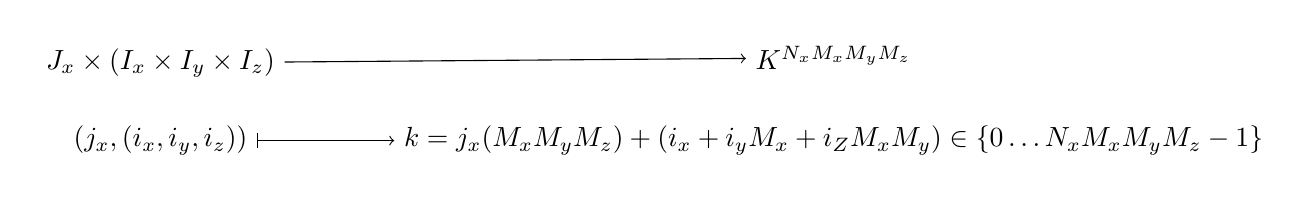
\begin{tikzpicture}
		\matrix (m) [matrix of math nodes, row sep=1.1em, column sep=4em, minimum width=1em]
		{
			J_x \times (I_x\times I_y \times I_z) &  K^{N_xM_xM_yM_z}  \\ 
			(j_x,(i_x,i_y,i_z)) & k = j_x(M_xM_yM_z) +(i_x+i_yM_x + i_Z M_xM_y)  \in \lbrace 0 \dots N_xM_xM_yM_z -1 \rbrace \\ 
		};
		\path[->]
		(m-1-1) edge node [auto] {$$} (m-1-2)
		;  
		\path[|->]
		(m-2-1) edge node [auto] {$$} (m-2-2)
		;
	\end{tikzpicture}
	\]
	\item  \emph{2-dim. grid} of \emph{1-dim. blocks}
	\[
	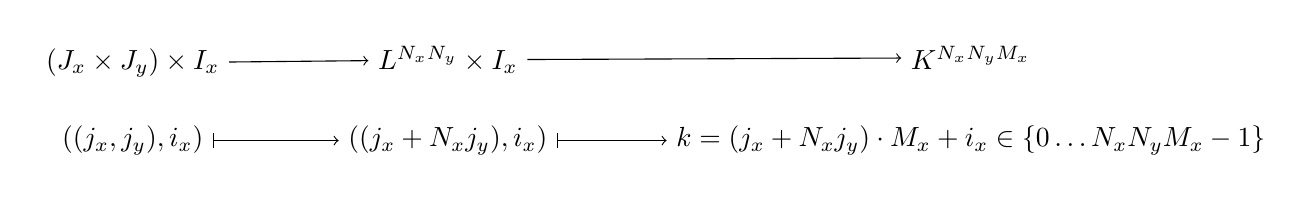
\begin{tikzpicture}
		\matrix (m) [matrix of math nodes, row sep=1.1em, column sep=4em, minimum width=1em]
		{
			(J_x\times J_y) \times I_x &  L^{N_xN_y} \times I_x & K^{N_xN_yM_x}  \\ 
			((j_x,j_y), i_x ) & ((j_x+N_xj_y) , i_x ) & k = (j_x + N_xj_y)\cdot M_x + i_x \in \lbrace 0 \dots N_xN_yM_x - 1 \rbrace   \\ 
		};
		\path[->]
		(m-1-1) edge node [auto] {$$} (m-1-2)
		(m-1-2) edge node [auto] {$$} (m-1-3) 
		;  
		\path[|->]
		(m-2-1) edge node [auto] {$$} (m-2-2)
		(m-2-2) edge node [auto] {$$} (m-2-3)
		;
	\end{tikzpicture} 
	\]
	\item \emph{2-dim. grid} of \emph{2-dim. blocks}
	\[
	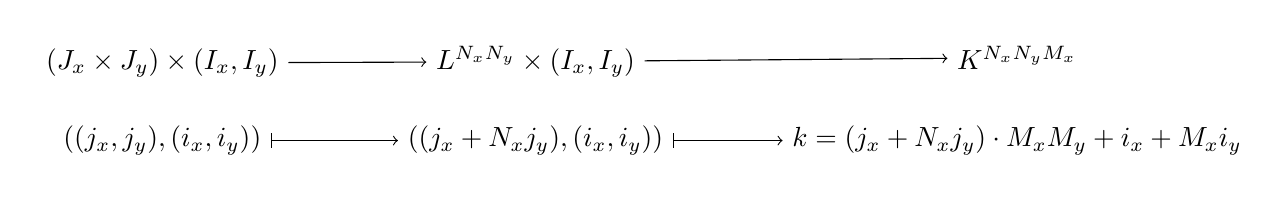
\begin{tikzpicture}
		\matrix (m) [matrix of math nodes, row sep=1.1em, column sep=4em, minimum width=1em]
		{
			(J_x\times J_y) \times (I_x,I_y) &  L^{N_xN_y} \times (I_x,I_y) & K^{N_xN_yM_x}  \\ 
			((j_x,j_y), (i_x,i_y) ) & ((j_x+N_xj_y) , (i_x,i_y) ) & k = (j_x + N_xj_y)\cdot M_xM_y + i_x +M_xi_y     \\ 
		};
		\path[->]
		(m-1-1) edge node [auto] {$$} (m-1-2)
		(m-1-2) edge node [auto] {$$} (m-1-3) 
		;  
		\path[|->]
		(m-2-1) edge node [auto] {$$} (m-2-2)
		(m-2-2) edge node [auto] {$$} (m-2-3)
		;
	\end{tikzpicture} 
	\] 
	But this \emph{isn't the only way of obtaining} a ``flattened index.''  Exploit the commutativity and associativity of the Cartesian product:
	\[
	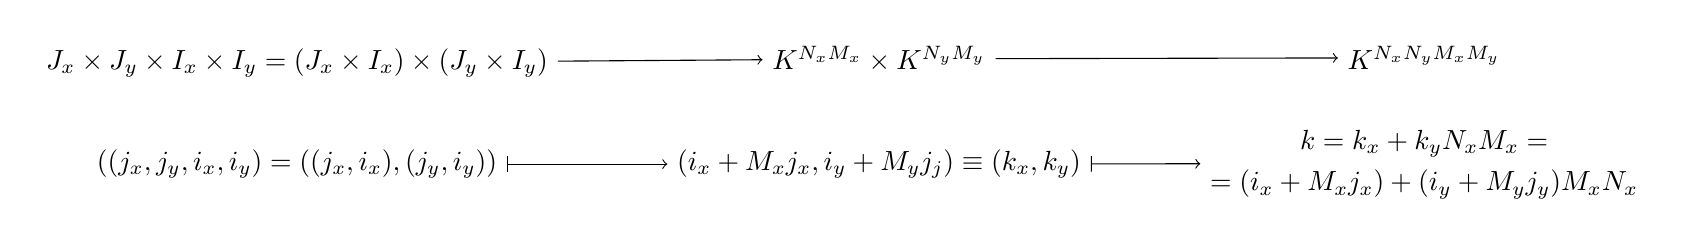
\begin{tikzpicture}
		\matrix (m) [matrix of math nodes, row sep=1.1em, column sep=4em, minimum width=1em]
		{
			J_x\times J_y \times I_x \times I_y = (J_x \times I_x) \times (J_y \times I_y) &  K^{N_xM_x} \times K^{N_yM_y}   & K^{N_xN_yM_xM_y}  \\ 
			((j_x,j_y,i_x,i_y ) = ((j_x,i_x),(j_y,i_y)) & (i_x+M_xj_x,i_y+M_yj_j)\equiv (k_x,k_y)  & \begin{gathered} k = k_x + k_yN_xM_x = \\ = (i_x+M_xj_x)+(i_y+M_yj_y)M_xN_x  \end{gathered}   \\ 
		};
		\path[->]
		(m-1-1) edge node [auto] {$$} (m-1-2)
		(m-1-2) edge node [auto] {$$} (m-1-3) 
		;  
		\path[|->]
		(m-2-1) edge node [auto] {$$} (m-2-2)
		(m-2-2) edge node [auto] {$$} (m-2-3)
		;
	\end{tikzpicture} 
	\] 
	Indeed, checking the ``maximal, extreme'' case,
	\[
	k = k_x + k_y N_xM_x = M_xN_x-1 + (M_yN_y - 1)(N_xM_x) = M_yM_yN_xM_x -1
	\]
	and so $k$ ranges from $0$ to $M_yM_yN_xM_x -1$.
		
	\item \emph{3-dim. grid} of \emph{3-dim. blocks}
	\[
	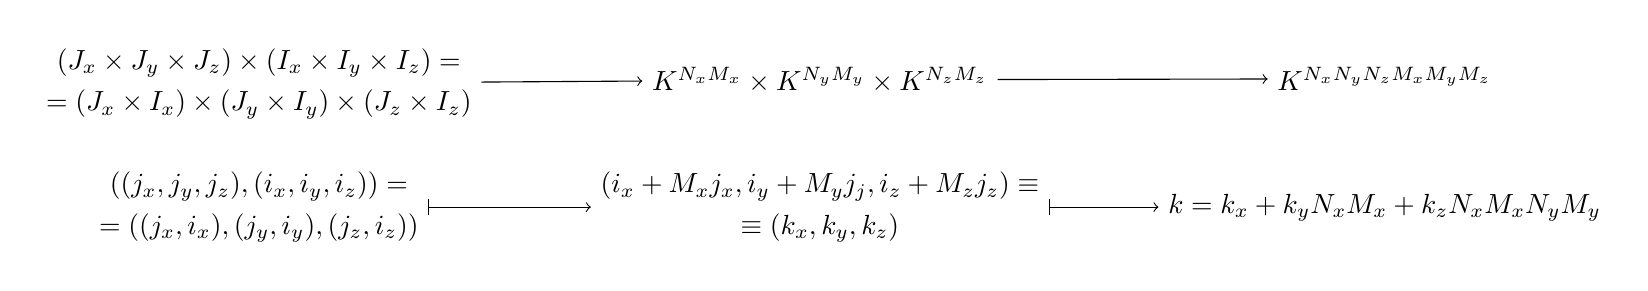
\begin{tikzpicture}
		\matrix (m) [matrix of math nodes, row sep=1.1em, column sep=4em, minimum width=1em]
		{
			\begin{gathered} (J_x\times J_y \times J_z ) \times (I_x \times I_y \times I_z) = \\
				= (J_x \times I_x) \times (J_y \times I_y) \times (J_z \times I_z) \end{gathered} &  K^{N_xM_x} \times K^{N_yM_y} \times K^{N_zM_z}   & K^{N_xN_yN_zM_xM_yM_z}  \\ 
			\begin{gathered} ((j_x,j_y,j_z),(i_x,i_y,i_z )) = \\ = ((j_x,i_x),(j_y,i_y),(j_z,i_z)) \end{gathered} & \begin{gathered} (i_x+M_xj_x,i_y+M_yj_j,i_z + M_zj_z)\equiv \\
				\equiv (k_x,k_y,k_z) \end{gathered}  & \begin{gathered} k = k_x + k_yN_xM_x + k_zN_xM_xN_yM_y    \end{gathered}   \\ 
		};
		\path[->]
		(m-1-1) edge node [auto] {$$} (m-1-2)
		(m-1-2) edge node [auto] {$$} (m-1-3) 
		;  
		\path[|->]
		(m-2-1) edge node [auto] {$$} (m-2-2)
		(m-2-2) edge node [auto] {$$} (m-2-3)
		;
	\end{tikzpicture} 
	\] 
	Indeed, checking the ``extreme, maximal'' case for $k$:
	\[
	\begin{gathered}
		k =   k_x + k_y N_xM_x + k_zN_xM_xN_yN_y = \\
		= (N_xM_x-1) + (N_yM_y-1)N_xM_x + (N_zM_z-1)N_xM_xN_yM_y = N_xN_yN_zM_xM_yM_z -1
	\end{gathered}
	\]
\end{itemize}

\subsection{With Stride}

Consider this code for the \href{https://github.com/NVlabs/tiny-cuda-nn/blob/master/include/tiny-cuda-nn/losses/l1.h}{L1 loss function} and \href{https://github.com/NVlabs/tiny-cuda-nn/blob/master/include/tiny-cuda-nn/losses/l2.h}{L2 loss function}. It introduces the idea of a "stride." Let's figure out what the stride means mathematically.

Given Eq. \ref{Eq:GlobalIndexCUDA1Dim}, recall that
\[
\begin{gathered}
k = j_x + i_x M_x, \quad \quad \, \begin{aligned} & 0 \leq j_x < M_x \\ & 0 \leq i_x < N_x \end{aligned}, \quad \, 0 \leq k < N_x M_x
\end{gathered}
\]

Let $S \equiv $ stride. 

Following the code we mentioned above for L1 and L2 loss functions, it seems that the following 2 indices were introduced, with inter roughly meaning "outside" or "outward" and intra meaning "within" or "internal", presumably:

\[
\begin{aligned}
	i_{\text{intra}} = k \mod{S} \in \lbrace 0, 1, \dots S-1 \rbrace \\
	i_{\text{inter}} = \lfloor k/ S \rfloor \in \lbrace 0 ,1, \dots (N_x M_x - 1) / S \rbrace
\end{aligned}
\]

Now let $D= $ number of dimensions.

Continuing with the code, it seems that $i_{\text{intra}} < D$ is what's expected. Otherwise, if $i_{\text{intra}} \geq D$, then we effectively don't compute.

\[
\begin{gathered}
	l \equiv i_{\text{inter}} D + i_{\text{intra}}, \quad \, 0 \leq l \leq \left( \frac{N_x M_x - 1}{S} \right)D + S -1
\end{gathered}
\]

Let's try some examples. If $S = 1$, $i_{\text{intra}} = 0$, always (the modulus of a number by 1 is always 0 because any number can be divided by 1 "evenly" (no remainder)), and $i_{\text{inter}} = k$. So $l = kD$. If $D=1$ we get a 1 to 1 mapping which is what I'd typically expect if given arrays. If $D=2$, then $l$ would be all the even indices it seems implied that the "target" array that's using $l$ as an index would have at least twice the size of the input array!

If $S=2$, $i_{\text{intra}} \in \lbrace 0 , 1\rbrace$, $i_{\text{inter}} \in \lbrace 0 ,1, \dots \lfloor \frac{N_x M_x - 1}{2} \rfloor \rbrace$ and so $l \in \lbrace 0,1, \dots \left( \frac{N_x M_x - 1}{2} \right) D + 1 \rbrace$. 


\section{Row-Major ordering vs. Column Major ordering, as flatten}

So-called row-major ordering and column major ordering should be formalized, to deal with continguous memory access in reading or writing to a matrix, or lack thereof.  

Given 
\[
\begin{gathered}
	A \in \text{Mat}_{\mathbb{R}}(m,n) \\ 
	\begin{aligned}
		& A: \lbrace 1,2, \dots m \rbrace \times \lbrace 1,2, \dots n \rbrace \to \mathbb{R} \\
		& A: (i,j) \mapsto A(i,j) \in \mathbb{R} 
	\end{aligned} \\
	\text{ or } 
	\begin{aligned}
		& A: \lbrace 0,1, \dots m-1 \rbrace \times \lbrace 0,1, \dots n-1 \rbrace \to \mathbb{R} \\
		& A: (i,j) \mapsto A(i,j) \in \mathbb{R} 
	\end{aligned} 
\end{gathered}
\]

Consider isomorphism "flatten":
\begin{equation}
	\begin{aligned}
		\text{Mat}_{\mathbb{R}}(m,n)  & \xrightarrow{\text{flatten} } \mathbb{R}^{mn} \\
		\lbrace 1,2, \dots m \rbrace  & \times \lbrace 1,2, \dots n \rbrace \to \lbrace 1,2,\dots mn \rbrace \\
		\lbrace 0,1, \dots m-1 \rbrace  & \times \lbrace 0,1, \dots n-1 \rbrace \to \lbrace 0,1,\dots mn-1 \rbrace
	\end{aligned}
\end{equation}

There are 2 kinds of flatten:

Row-major ordering is the one we're (psychologically) used to, if we read continguously from left to right, horizontally, along a row.  
\begin{definition}[row-major ordering]
	\begin{equation}
		\begin{gathered}
			\begin{gathered}
				\lbrace 0,1, \dots m-1 \rbrace \times \lbrace 0,1, \dots n-1 \rbrace \to \lbrace 0,1,\dots mn-1 \rbrace  \\
				(i,j ) \mapsto in + j \\
				\lbrace 1,2, \dots m \rbrace \times \lbrace 1,2, \dots n \rbrace \to \lbrace 1,2,\dots mn \rbrace \\
				(i,j) \mapsto (i-1)n + j 
			\end{gathered}
			\qquad \  \begin{gathered}
				\lbrace 0,1,\dots mn-1 \rbrace \to \lbrace 0,1, \dots m-1 \rbrace \times \lbrace 0,1, \dots n-1 \rbrace \\
				k \mapsto (k/n, k \mod{n}) \\ 
				\lbrace 1,2,\dots mn \rbrace \to \lbrace 1,2, \dots m \rbrace \times \lbrace 1,2, \dots n \rbrace  \\
				k \mapsto ( \lceil k/n \rceil, k \mod{n})
			\end{gathered}
		\end{gathered}
	\end{equation}
\end{definition}

\begin{definition}[column-major ordering]
	\begin{equation}
		\begin{gathered}
			\begin{gathered}
				\lbrace 0,1, \dots m-1 \rbrace \times \lbrace 0,1, \dots n-1 \rbrace \to \lbrace 0,1,\dots mn-1 \rbrace  \\
				(i,j ) \mapsto i + jm \\
				\lbrace 1,2, \dots m \rbrace \times \lbrace 1,2, \dots n \rbrace \to \lbrace 1,2,\dots mn \rbrace \\
				(i,j) \mapsto i + (j-1)m 
			\end{gathered}
			\qquad \  \begin{gathered}
				\lbrace 0,1,\dots mn-1 \rbrace \to \lbrace 0,1, \dots m-1 \rbrace \times \lbrace 0,1, \dots n-1 \rbrace \\
				k \mapsto (k \mod{m}, k/m) \\ 
				\lbrace 1,2,\dots mn \rbrace \to \lbrace 1,2, \dots m \rbrace \times \lbrace 1,2, \dots n \rbrace  \\
				k \mapsto ( k \mod{m} , \lceil k/ m \rceil )
			\end{gathered}
		\end{gathered}
	\end{equation}
\end{definition}

\part{Embeddings}

\section{FAISS}



\end{multicols*}
\begin{thebibliography}{9}
\bibitem{HTF2009}
Trevor Hastie, Robert Tibshirani, Jerome Friedman.   \textbf{The Elements of Statistical Learning: Data Mining, Inference, and Prediction}, Second Edition (Springer Series in Statistics) 2nd ed. 2009. Corr. 7th printing 2013 Edition.  ISBN-13: 978-0387848570.  \url{https://web.stanford.edu/~hastie/local.ftp/Springer/OLD/ESLII_print4.pdf}

\bibitem{CS2013}
Jared Culbertson, Kirk Sturtz.  \emph{Bayesian machine learning via category theory}.  \href{http://arxiv.org/abs/1312.1445}{arXiv:1312.1445} [math.CT]

\bibitem{CS344}
John Owens.  David Luebki.  \emph{Intro to Parallel Programming}.  \emph{CS344}.  \textbf{\href{https://www.udacity.com/}{Udacity}}  
  
\url{http://arxiv.org/abs/1312.1445} Also, \url{https://github.com/udacity/cs344}  

\bibitem{CS229}
CS229 Stanford University.  \url{http://cs229.stanford.edu/materials.html}


\bibitem{Fitz}
Richard Fitzpatrick.  ``Computational Physics.''  \url{http://farside.ph.utexas.edu/teaching/329/329.pdf}

\bibitem{LISA2015}
LISA lab, University of Montreal.  Deep Learning Tutorial.  \url{http://deeplearning.net/tutorial/deeplearning.pdf}  September 2015.  



\bibitem{Horn1991}
Kurt Hornik. ``Approximation Capabilities of Muitilayer Feedforward Networks.''  \textbf{Neural Networks}, Vol. 4, pp. 251-257. 1991

\bibitem{HSW1989}
Kurt Hornik. Maxwell Stinchcombe and Halbert White.  ``Multilayer Feedforward Networks are Universal Approximators.''  \textbf{Neural Networks}, Vol. 2, pp. 359-366, 1989.  


\bibitem{JZS2015}
Rafal Jozefowicz, Wojciech Zaremba, Ilya Sutskever.  "An Empirical Exploration of Recurrent Network Architectures."  \emph{Proceedings of the 32 nd International Conference on Machine Learning}, Lille, France, 2015. JMLR: W\&CP volume 37.

\bibitem{GBC2016}
Ian Goodfellow, Yoshua Bengio, and Aaron Courville.  \textbf{Deep Learning} (Adaptive Computation and Machine Learning series).  The MIT Press (November 18, 2016).  


% EY : 20171024  
\bibitem{BrCh2016}
Jacob C. Bridgeman, Christopher T. Chubb.  \emph{Hand-waving and Interpretive Dance: An Introductory Course on Tensor Networks}.  
\href{arXiv:1603.03039}{https://arxiv.org/abs/1603.03039} [quant-ph]


\bibitem{Stut2014}
David Stutz.  \emph{Understanding Convolutional Neural Networks}.  Seminar Report.  August 30, 2014.  Advisor: Lucas Beyer.  Fakultät für Mathematik, Informatik und Naturwissenschaften; Lehr- und Forschungsgebiet Informatik VIII; Computer Vision; Prof. Dr. Bastian Leibe.  \url{http://davidstutz.de/wordpress/wp-content/uploads/2014/07/seminar.pdf}.  

\bibitem{LaGr2015}  
Andrew Lavin, Scott Gray.  \emph{Fast Algorithms for Convolutional Neural Networks} \href{https://arxiv.org/abs/1509.09308}{arXiv:1509.09308 [cs.NE]}

\bibitem{Nowa2008}
Thomas Nowak.  ``Implementation and Evaluation of a Support Vector Machine on an 8-bit Microcontroller.''  Univ.Ass. Dipl.-Ing. Dr.techn. Wilfried Elmenreich Institut f\"{u}r Technische Informatik Fakult\"{a}t f\"{u}r Informatik Technische Universit\"{a}t Wien.  Juli 2008.  \url{https://www.lri.fr/~nowak/misc/bakk.pdf}

\bibitem{STCr2000}
J.  Shawe-Taylor  and  N.  Cristianini,  Support  Vector  Machines  and  other  kernel-based  learning  methods,
Cambridge University Press (2000).

\bibitem{ChZa2013}
Edwin K. P. Chong and Stanislaw H. Zak.  \textbf{An Introduction to Optimization}.  4th Edition.  Wiley.  (January 14, 2013).  ISBN-13: 978-1118279014
  
\bibitem{Nara2015}
Lecture by Harikrishna Narasimhan.  \emph{Optimization Tutorial 3: Projected Gradient Descent, Duality}.  \textbf{E0 270 Machine Learning}.  Jan 23, 2015.  \url{http://drona.csa.iisc.ernet.in/~e0270/Jan-2015/Tutorials/lecture-notes-3.pdf}

\bibitem{Bish2007}
Christopher M. Bishop.  \textbf{Pattern Recognition and Machine Learning} (Information Science and Statistics).  Springer (October 1, 2007).  ISBN-13: 978-0387310732


\bibitem{CFZ2009}
Bertrand Clarke, Ernest Fokoue, Hao Helen Zhang.   \textbf{Principles and Theory for Data Mining and Machine Learning} (Springer Series in Statistics)  Springer; 2009 edition (July 30, 2009).  ISBN-13: 978-0387981345
 

\bibitem{Ngu2007}
Hubert Nguyen. \textbf{GPU Gems 3}.  Addison-Wesley Professional (August 12, 2007).  ISBN-13: 978-0321515261.  Also made available in its entirety online at \url{https://developer.nvidia.com/gpugems/GPUGems3/gpugems3_pref01.html}

\bibitem{Pedr2011}
  Scikit-learn: Machine Learning in Python, Pedregosa \emph{et al.}, \textbf{JMLR 12}, pp. 2825-2830, 2011.


\bibitem{CySi2009}
Bogus\l{} aw Cyganek.  J. Paul Siebert.  \textbf{An Introduction to 3D Computer Vision Techniques and Algorithms}.  Wiley.  2009.  ISBN 978-0-470-01704-3

 \bibitem{HaZi2003}
Richard Hartley.  Andrew Zisserman.  \textbf{Multiple View Geometry in Computer Vision}  Second Edition.  \emph{Cambridge University Press.}  2003.  ISBN-13 978-0-511-18618-9 eBook (EBL)

\bibitem{JLee2012}
John Lee, \textbf{Introduction to Smooth Manifolds} (Graduate Texts in Mathematics, Vol. 218), 2nd edition, Springer,  2012, ISBN-13: 978-1441999818

\bibitem{JLee2009}
Jeffrey M. Lee. \textbf{Manifolds and Differential Geometry}, \emph{Graduate Studies in Mathematics} Volume: 107, American Mathematical Society, 2009. ISBN-13: 978-0-8218-4815-9



\bibitem{ChLi2011}
  C.-C. Chang and C.-J. Lin. \emph{LIBSVM : a library for support vector machines}. \textbf{ACM Transactions on Intelligent Systems and Technology}, 2:27:1--27:27, 2011. 

\bibitem{Pla1998}
  J. Platt. \emph{Fast training of support vector machines using sequential minimal optimization}. In A. Smola B. Schölkopf, C. Burges, editor, \textbf{Advances in Kernel Methods: Support Vector Learning}. MIT Press, Cambridge, MA, 1998.

\bibitem{HCL}
Chih-Wei Hsu, Chih-Chung Chang, and Chih-Jen Lin.  \emph{A Practical Guide to Support Vector Classification}.  \url{http://www.ee.columbia.edu/~sfchang/course/spr/papers/svm-practical-guide.pdf}

\bibitem{MiTa}
Rada Mihalcea and Paul Tarau.  "TextRank: Bringing Order into Texts."  
\url{https://web.eecs.umich.edu/~mihalcea/papers/mihalcea.emnlp04.pdf}  

\bibitem{Glei2015}
David F. Gleich.  \emph{PageRank Beyond the Web.}  \textbf{SIAM Review}.  Vol. 57, No. 3, pp. 321-363 2015  
  
\bibitem{PBMW1998}  
Page, Lawrence and Brin, Sergey and Motwani, Rajeev and Winograd, Terry.  "The PageRank Citation Ranking: Bringing Order to the Web." Technical Report. Stanford InfoLab.  1998.  \url{http://ilpubs.stanford.edu:8090/422/1/1999-66.pdf}  
  
\bibitem{TUMHPC2016}
Prof. Dr. Michael Bader, with Alexander P\"{o}ppl, Valeriy Khakhutskyy (Tutorials).  High Performance Computing (HPC) - Algorithms and Applications - Winter 16/17.  Informatics V - Scientific Computing.  Technical University of Munich (TUM)
\url{https://www5.in.tum.de/wiki/index.php/HPC_-_Algorithms_and_Applications_-_Winter_16}


\bibitem{AnNg}
Andrew Ng.  \href{https://www.coursera.org/learn/machine-learning/home/welcome}{Machine Learning}.  \href{https://www.coursera.org}{coursera}


\bibitem{StBe1999}
Kilian Stoffel and Abdelkader Belkoniene.  \emph{Parallel $k/h$-Means Clustering for Large Data Sets}.  Euro-Par'99, LNCS 1685, pp. 1451-1454, 1999.  Springer-Verlag Berlin Heidelberg 1999

\url{https://grid.cs.gsu.edu/~wkim/index_files/papers/parkh.pdf}

\bibitem{theano}
Theano Development Team. \href{http://arxiv.org/pdf/1605.02688.pdf}{“Theano: A Python framework for fast computation of mathematical expressions”}. 

\bibitem{JRotman2010}
Joseph J. Rotman, \textbf{Advanced Modern Algebra} (Graduate Studies in Mathematics) 2nd Edition, American Mathematical Society; 2 edition (August 10, 2010), ISBN-13: 978-0821847411

\bibitem{JLee2009}
Jeffrey M. Lee. \textbf{Manifolds and Differential Geometry}, \emph{Graduate Studies in Mathematics} Volume: 107, American Mathematical Society, 2009. ISBN-13: 978-0-8218-4815-9

\bibitem{Conl2008}
Lawrence Conlon.  \textbf{Differentiable Manifolds} (Modern Birkhäuser Classics).  2nd Edition.  Birkhäuser; 2nd edition (October 10, 2008).  ISBN-13: 978-0817647667

\bibitem{SageMath2017}
The Sage Development Team.  Sage Reference Manual: Category Framework.  Release 7.6.  Mar. 25, 2017.  

\bibitem{tensorflow2015}
Martín Abadi, Ashish Agarwal, Paul Barham, Eugene Brevdo,Zhifeng Chen, Craig Citro, Greg S. Corrado, Andy Davis,Jeffrey Dean,Matthieu Devin, Sanjay Ghemawat, Ian Goodfellow,Andrew Harp, Geoffrey Irving, Michael Isard, Rafal Jozefowicz, Yangqing Jia,Lukasz Kaiser, Manjunath Kudlur, Josh Levenberg, Dan Mané, Mike Schuster,Rajat Monga, Sherry Moore, Derek Murray, Chris Olah, Jonathon Shlens,Benoit Steiner, Ilya Sutskever, Kunal Talwar, Paul Tucker,Vincent Vanhoucke, Vijay Vasudevan, Fernanda Viégas,Oriol Vinyals, Pete Warden, Martin Wattenberg, Martin Wicke,Yuan Yu, and Xiaoqiang Zheng.  
\emph{TensorFlow: Large-scale machine learning on heterogeneous systems}, 2015. Software available from \href{http://tensorflow.org/}{tensorflow.org.}

\bibitem{JZS2015}
Rafal Jozefowicz, Wojciech Zaremba, Ilya Sutskever.  "An Empirical Exploration of Recurrent Network Architectures."  \emph{Proceedings of the 32nd
International  Conference on  Machine Learning}, Lille, France, 2015.  JMLR: W\&CP volume 37.  \url{http://www.jmlr.org/proceedings/papers/v37/jozefowicz15.pdf} 

\bibitem{SK2010}
Jason Sanders, Edward Kandrot.  \textbf{CUDA by Example: An Introduction to General-Purpose GPU Programming} 1st Edition.  Addison-Wesley Professional; 1 edition (July 29, 2010).  ISBN-13: 978-0131387683
  
\end{thebibliography}

\end{document}
